\chapter{Design}
\label{ch:design}
% report goes here

\section{Educational Design Decisions}

\section{Game Design}
The aim of our game design was to efficiently encode collaborative learning in the mechanics of the game. This section will list and describe all the additional elements that we decided to add to the existing Minecraft 1.6.4 core game in order to create a playable mod that would fulfill our requirements. We gradually introduced new elements as and when required.
\newline\newline
The mod is set to be played in adventure mode\footnote{``Adventure mode is a game mode intended for player-created maps by limiting some of the gameplay in Minecraft, in which the player cannot directly destroy most blocks to avoid spoiling adventure maps or griefing servers. Most blocks cannot be destroyed without the proper tools. However, players can still interact with mobs and craft items.''\cite{website:minecraft-adventure}}.
We have tried to preserve as much of the Minecraft concepts in our extension as possible, so that players familiar with the game can easily understand the mechanics of our mod. Inexperienced users will also get to know the Minecraft philosophy whilst using our extension and will be able to play the original game or some other mods without any problems in the future.

\subsection[Items]{Items\footnote{``Items are objects which only exist within the player's inventory and hands - which means, they cannot be placed in the game world. Some items simply place blocks or entities into the game world when used. They are thus an item when in the inventory and a block when placed.''\cite{website:minecraft-item}}}

\begin{itemize}

\item \textbf{Numbers}
\newline
\normalsize These are the most important element in our extension and are crucial for promoting the practice of mathematics. Numbers are used in several of the features our mod offers.

\item \textbf{Operators}
\newline
\normalsize Operators are as important as numbers, but only used in certain parts of the mod and are key elements of performing arithmetic operations.

\item \textbf{Keys}
\newline
\normalsize Keys are used for progressing in the game. They allow us to place constraints on the free movement of players.

\item \textbf{Maths Wands}
\newline
\normalsize Maths Wands enable us to limit the choice of weapons used for killing mobs.

\end{itemize}

\subsection[Blocks]{Blocks\footnote{``Blocks are the basic units of structure in Minecraft, and are essential to the gameplay. Together, they build up the in-game environment and can be utilized in various fashions.''\cite{website:minecraft-blocks}}}

\begin{itemize}
\large \item \textbf{Crafting Table}\footnote{``The Crafting Table (or Workbench) is one of the most essential blocks in Minecraft. Right-clicking on a crafting table placed in the world will open the 3×3 crafting grid which allows you to craft more items than with the crafting grid in your inventory. A crafting table is essential in order to progress at all in the game.''\cite{website:minecraft-table}}

\normalsize
\begin{itemize}
\item \textbf{Operator Bench}
\newline
\normalsize This is a slightly modified version of the Crafting Table and it is used for creating mathematical operators from sticks.	

\item \textbf{Ordering Bench}
\newline
\normalsize This is a modified version of the Crafting Table which only accepts numbers as inputs. It requires the players to order the input numbers in order to generate an output. It has three different subtypes accepting all, only odd or only even numbers.

\item \textbf{Calculator Bench}
\newline
\normalsize This is a modified version of the Crafting Table which only accepts numbers and operators as inputs. It allows the players to generate new numbers from the inputs. It performs simple arithmetic operations based on the type of the operator in the input matrix.
\end{itemize}
\end{itemize}

\subsection[Mobs]{Mobs\footnote{``Mobs are living, moving game entities. Generally, mobs are affected by the environment in the same ways as the player: they are subject to physics, and they can be hurt by almost all the same things that harm the player: Catching on fire, falling, drowning or suffocating, and of course being attacked with weapons.''\cite{website:minecraft-mobs}}}

\begin{itemize}
\item \textbf{Zombies}
\newline
\normalsize This modified version of the original Zombie hostile mob can only be killed by using Math Wands and they drop numbers when slayed.

\item \textbf{Skeletons}
\newline
\normalsize This is a modified version of the original Skeleton hostile with similar properties to Zombies. Skeletons are armed with bows that shoot arrows at the player. This makes them more difficult to kill.
\newline
\end{itemize}

\section{Level Design}
There are no levels in Minecraft, so we decided to create different locations representing the levels. The locations will also be referred to as levels in the rest of this report. The levels are used for controlling the learning experience of the players. Levels are a form of constraint that we have managed to utilise to create a learning curve within the game.
\newline\newline
Level design decisions were deliberately made to ensure collaboration between players as well as encouraging communication. Researches show that communication and collaboration are linked and can improve the process of learning within groups.
Most of the advanced levels consist of a mixture of easy and hard tasks. The purpose of this variety is to make the levels hard enough to engage the players and let them enjoy playing without making the game too hard to progress which would eventually result in the players losing interest.
\newline\newline
Even though our mod does not have a storyline which would add a fantasy context to the gameplay, our location designs are based on recognisable historical architectures. Our initial world was completely flat, but we have created various landscapes in the vicinity of our locations to improve the visual experience in the mod. We wanted to show that Minecraft has the potential to implement a wide range of design ideas.

\subsection{Locations}

\begin{itemize}
\item \textbf{Concept of a room}\newline
A “room” is an abstract concept, that we used throughout the development process. It is used for controlling the free movement of the players in the world and to synchronize the collaborative progress of the team or subteams. Some of the initial tests with children showed that they tend to walk around aimlessly to discover new parts of the world, which results in losing focus on the tasks to be completed.
The room consists of an entrance and an exit. In most rooms once the player enters they cannot return to previous parts of the world. The room can only be exited once a specific task is completed.

\item \textbf{Castle}\newline
The Castle requires players to collaborate and work as a group of four. This level is designed to teach the players how to play the mod and could also be considered as the tutorial level of the game. The players are introduced to the concept of a room and learn how to create operators, use various benches and obtain numbers.

\item \textbf{Pyramid}\newline
The Pyramid level splits the players into two sub teams of two. There are various elements in this level that require good communication between the players in order to collaboratively progress through to the end of this level. There are limitations on the resources accessible to both teams, hence ``no one can win without the help of the others''. Ordering, subtraction and addition are the only mathematical operations required in this location.

\item \textbf{Rook}\newline
The Rook implements the same principles as the Pyramid. The only difference is in the type of mathematical operations set as tasks, which are multiplication and division for this level.\newline
\end{itemize}
\begin{figure}[H]
\centering
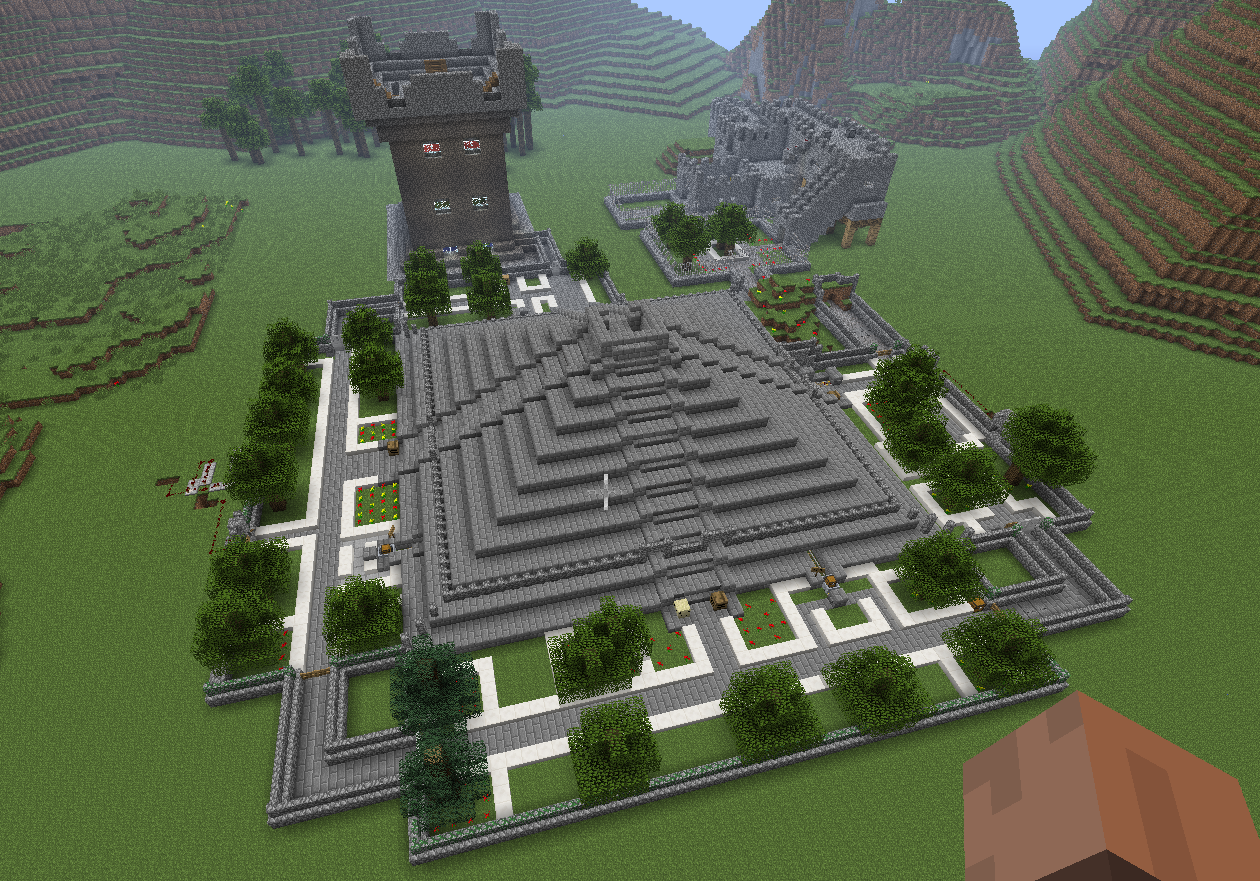
\includegraphics[scale=0.5]{locations}
\caption{"Screenshot of the EduCraft world"}
\end{figure}